\documentclass[12pt]{article}

\def\pdfpsfrag{no}
\def\reusepsfragpdf{yes or no}
\def\foiltex{no}
\def\algfontmode{no}
\input{../../FrequentlyUsed/latex/mydefs}

\usepackage{fullpage}
\usepackage{tikz}
\usetikzlibrary{decorations.pathreplacing}

\title{Dynamics systems in Physics}
\author{Sunghee Yun - Beth's Daddy \& Liam, Lucy, Adrian \& Lillian's Uncle}

\begin{document}
\maketitle
\tableofcontents

\newpage
\section{Force equations}

\subsection{Ideal springs}

Suppose (simple) rules for springs hold. That is when a spring with $k\in\ppreals$ as the spring constant and $l\in\ppreals$ as the natural length
and two point masses $m_1\in\ppreals$ and $m_2\in\ppreals$, which are located at
$x_1\in\reals^3$
and
$x_2\in\reals^3$
as show in \figurename~\ref{fig:spring}.
The force exerted on $m_1$ is
\begin{equation}
\label{eq:force:spring}
	F_s(x_1;k,l,x_2) = -k (\|x_1-x_2\| - l) v_{2,1}
	= -k
	\left(
	\frac{\|x_1-x_2\| - l}{\|x_1-x_2\|}
	\right)
	(x_1-x_2)
\end{equation}
where $v_{2,1}\in\reals^3$ is a unit-length vector pointing to the direction of $x_1-x_2$,
\ie,
\[
	v_{2,1} =
%	\left(
	\frac{1}{\|x_1-x_2\|}
%	\right)
	(x_1-x_2).
\]
Here $\|x\|$ is the $2$-norm or the size of a vector $x\in\reals^3$ defined by
\[
	\|x\| = \sqrt{x_1^2+x_2^2+x_3^2}.
\]

The force exerted on $m_2$ $F_s(x_2;k,l,x_1)$ be can obtained using 

\begin{figure}
\begin{center}
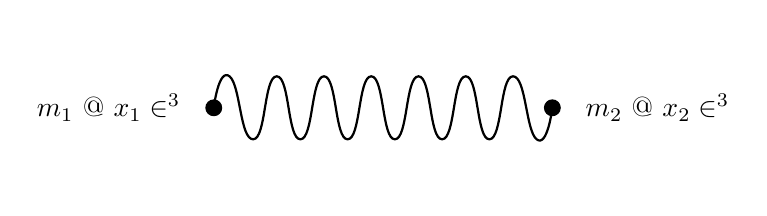
\begin{tikzpicture}[scale=1]
\def\coils{6} % Number of coils
\def\radius{0.4} % Radius of coils
\def\length{5} % Total length of spring
\def\startx{-2} % Starting x coordinate
\def\starty{0} % Starting y coordinate
\def\slope{2} % Height increase over length

%    \draw[very thin, dashed] (-3.5, -1) rectangle (3.8, 1); % Rectangle boundary
	\node[inner sep=0pt, outer sep=0pt] (left) at (-3.5, 0) {};
    \node[inner sep=0pt, outer sep=0pt] (right) at (3.8, 0) {};
    \node[inner sep=0pt, outer sep=0pt] (top) at (0, 1) {};
    \node[inner sep=0pt, outer sep=0pt] (bottom) at (0, -1) {};
    % Draw balls

	\def\ballo{(-2, 0)}
    \def\ballt{(2.3, 0)}
    
    % Draw balls
    \draw[fill=black] \ballo circle (0.1); % Ball 1
    \draw[fill=black] \ballt circle (0.1); % Ball 2

	\node[left=.3cm] at (-2, 0) {$m_1$ @ $x_1\in\reals^3$};
    \node[right=.3cm] at (2.3, 0) {$m_2$ @ $x_2\in\reals^3$};

\draw[thick] plot[smooth, tension=1]
  coordinates {
    (\startx+0.0,\starty)
    (\startx+0.2,\starty+\radius)
    (\startx+0.5,\starty-\radius)
    (\startx+0.8,\starty+\radius)
    (\startx+1.1,\starty-\radius)
    (\startx+1.4,\starty+\radius)
    (\startx+1.7,\starty-\radius)
    (\startx+2.0,\starty+\radius)
    (\startx+2.3,\starty-\radius)
    (\startx+2.6,\starty+\radius)
    (\startx+2.9,\starty-\radius)
    (\startx+3.2,\starty+\radius)
    (\startx+3.5,\starty-\radius)
    (\startx+3.8,\starty+\radius)
    (\startx+4.1,\starty-\radius)
    (\startx+4.3,\starty)
  };
\end{tikzpicture}
\end{center}
\caption{A spring connecting two point masses}
\label{fig:spring}
\end{figure}

\subsection{Gravity-like forces}

In a real world we live, we feel the gravity dragging us downward.
But since we can assume anything here! :)
let us assume that there exists gravity-like force
in a sense that given an acceleration vector $a\in\reals^3$,
the force exerted on a point mass $m\in\ppreals$ located at $x\in\reals^3$
is
\begin{equation}
\label{eq:force:gravity-like}
F_g(m;a) = ma
	\in\reals^3
\end{equation}
\ie,
the magnitude of the force is proportional to $m$ (and the magnitude of the acceleration),
the direction is the same as that of the acceleration.
It does \emph{not} depend on the location.

A typical example, of course, is \emph{the} gravity where
\[
	a = (0,0,-g)
	\in\reals^3
\]
with $g = 9.8 m/s^2$.

\subsection{Frictional forces}

We model frictional forces exerted on bodies (not point mass)
using the coefficient of friction $c\in\ppreals$ where the force is modeled by

\begin{equation}
\label{eq:force:frictional}
F_f(v) = -c v
	\in\reals^3
\end{equation}
where $v\in\reals^3$ is the velocity along the surface.

\section{Energies}

\subsection{Kinetic energy of a mass}

The kinetic energy of a mass $m$ with velocity $v\in\reals^3$
is defined by
\begin{equation}
\label{eq:energy:kinetic}
	E_\mathrm{k}(m) = \frac{m}{2} \|v\|^2
\end{equation}

\subsection{Potential energy}

Note that the role of the potential energies in dynamics
is played in a way that the difference of them at two location,
hence adding a constant to any potential energy
makes no difference.

\subsubsection{Potential energy by a gravity-like force}

The potential energy of a mass $m$ by a gravity-like force with acceleration $a\in\reals^3$
is defined by
\begin{equation}
\label{eq:energy:potential:gravity-like}
E_\mathrm{p,g}(m,x;a)
=  - m x\cdot a
= - m x^Ta
\end{equation}
where $a^Tb = a\cdot b$ for two vectors $a$ and $b$
is the inner product defined by
\[
	(a_1,a_2,a_3) \cdot (b_1,b_2,b_3) = a_1b_1 + a_2b_2 + a_3b_3.
\]
For example, the potential energy by gravity is
\[
	E_\mathrm{p,g}(m,x;g)
	= -(0,0,-g) \cdot (x_1,x_2,x_3)
	=  mgx_3
\]

\subsubsection{Potential energy by a spring}

The potential energy of a mass $m$ by a gravity-like force with acceleration $a\in\reals^3$
is defined by
\begin{equation}
\label{eq:energy:potential:spring}
E_\mathrm{p,s}(x_1,x_2;k,l)
= \frac{k}{2} (\|x_1-x_2\|-l)^2
\end{equation}


\subsection{The law of preservation of the energy}

In a system with masses, springs, and gravity-like forces with no frictional forces,
the sum of the kinetic energies of all the masses
and that of the potential energies of all the gravity-like forces and springs
is preserved
unless, for example, external forces are exerted on the system,
two point masses merge into one,
or some non-elastic crashes happen.

\subsubsection{Proof}
\label{subsubsection:proof}

Suppose that the location of a point mass $m$ is $x(t)\in\reals^3$
and the force exerted on $m$ is $F(t)\in\reals^3$ where $t$ refers to the time.
These notations explicitly show that both quantities are functions of time $t$.
The Newton's second law, $F(t) = m a(t)$ where $a(t) = \frac{d}{dt^2}x(t)$ is the acceleration of $m$,
implies
\begin{eqnarray}
\nonumber
\lefteqn{
\int_{t_1}^{t_2} (-F(t)) \cdot d x
 = - \int_{t_1}^{t_2} m a(t) \cdot d x
 = - \int_{t_1}^{t_2} m \left( \frac{dv(t)}{dt} \right) \cdot v(t) dt
}\\
 &=& - \int_{t_1}^{t_2} m {v(t)} \cdot dv(t)
= - \left(
 	\frac{m}{2}v(t_2)^2 - \frac{m}{2} v(t_1)^2
 \right)
=
\frac{m}{2} v(t_1)^2
- \frac{m}{2}v(t_2)^2
\label{eq:energy:preserve:1}
\end{eqnarray}
where we use the definition of velocity,
$v(t) = {dx(t)}/{dt}$.

Now we will show that $\int (-F(t)) dt $ is the same as (the difference of) the potential energies defined for
the gravity-like force and the spring respectively. 
For the gravity-like force,
we have
\begin{equation}
\label{eq:potential-energy-gravity-like}
	\int_{t_1}^{t_2} (-F(t))\cdot dx
=
	-m \int_{t_1}^{t_2} a\cdot dx
=
	-m (a\cdot x(t_2) - a\cdot x(t_1))
=
	E_\mathrm{p,g}(t_2)
	-
	E_\mathrm{p,g}(t_1).
\end{equation}
For the spring,
we have
\begin{equation}
\label{eq:potential-energy-gravity-like}
	\int_{t_1}^{t_2} (-F(t))\cdot dx
=
	\cdots
=
	E_\mathrm{p,s}(t_2)
	-
	E_\mathrm{p,s}(t_1).
\end{equation}

Therefore for any type of force,
(\ref{eq:energy:preserve:1})
implies
\begin{equation}
\label{eq:energy-preserve-for-each-mass}
E_\mathrm{p}(t_2) - E_\mathrm{p}(t_1)
=
\frac{m}{2} v(t_1)^2
- \frac{m}{2}v(t_2)^2
\Leftrightarrow
\frac{m}{2} v(t_1)^2 + E_\mathrm{p}(t_1)
=
\frac{m}{2} v(t_2)^2 + E_\mathrm{p}(t_2),
\end{equation}
hence the total energy,
\ie,
the sum of the kinetic energy and the potential energy,
is preserved for a point mass.

Because the potential energy is additive quantity
and (\ref{eq:energy-preserve-for-each-mass})
holds for each mass in a given system,
the law of the preservation of the energy hold
for a dynamic system satisfying the conditions mentioned above.


\subsection{Dissipated energy by a frictional force}

The energy dissipated due to a frictional force exerted on a mass
can be calculated by
\begin{equation}
\int F_f(v) \cdot dx
\end{equation}

\subsection{The law of preservation of the energy with frictional forces}

In a system with masses, springs, and gravity-like forces \emph{with} frictional forces,
the sum of the kinetic energies and potential energies is reduced
and the amount of reduction is (exactly) the same as the total dissipated energy.

\subsubsection{Proof}

It is quite straightforward to show this using similar derivations
used in \S\ref{subsubsection:proof},
thus we will now show it here.


\section{Momentum}

The momentum of a mass $m$ with velocity $v$ is defined by
\begin{equation}
M(m,v) = mv \in\reals^3
\end{equation}

\subsection{The law of preservation of the momentum}

In a system with masses,
the (vector) sum of the momentum of all the masses
is preserved
unless, for example, external forces are exerted on the system
even when, for example, two point masses merge into one or some non-elastic crashes happen.


\subsubsection{Proof}

Suppose a point mass $m$.
If no force is exerted, the momentum is (of course) preserved.

Now suppose two point masses $m_1$ and $m_2$.
If they exert forces on each other,
by the Newton's third law,
the forces exerted on each point mass
is the same in magnitude and the exact opposite in direction.
Assume that $F(t)\in\reals^3$ is exerted on $m_1$, then we have
\[
	\int_{t_1}^{t_2} F(t) dt
= \int_{t_1}^{t_2} m_1 a_1(t) dt
= \int_{t_1}^{t_2} m_1 dv_1(t)
= m_1v_1(t_2) - m_1 v_1(t_1)
\]
and
\[
	-\int_{t_1}^{t_2} F(t) dt
= \int_{t_1}^{t_2} m_2 a_2(t) dt
= \int_{t_1}^{t_2} m_2 dv_2(t)
= m_2v_2(t_2) - m_2 v_2(t_1)
\]
where we use $a(t) = dv(t) / dt$.
Adding these two equations give us
\begin{equation}
\label{eq:momemtum-preserved-for-two-masses}
m_1v_1(t_1) + m_2v_2(t_1)
=
m_1v_1(t_2) + m_2v_2(t_2).
\end{equation}
Therefore the (vector) sum of the momentums of two masses is preserved.

Now (\ref{eq:momemtum-preserved-for-two-masses}) holds for every interacting mass pairs,
the sum of the momentums of all the masses in a system is preserved
while the conditions mentioned above are satisfied.


\section{Equilibrium point}

An equilibrium point of a system
is defined by the configuration of all the masses in the system
so as to minimize the total energy
or equivalently, 
that where the force exerted on every mass, \ie, the sum of all the forces exerted on every mass,
is zero.


\subsection{Finding the equilibrium point}

For illustration,
suppose that there are two point masses
$m_1$ and $m_2$ whose locations are $x_1\in\reals^3$ and $x_2\in\reals^3$
and three springs with spring constants $k_i$ and natural lengths $l_i$ for $i=1,2,3$.
Assume one end of the first spring is fixed at $y_1$ and the other end is attached to $m_1$,
the second spring is attached to $m_1$ and $m_2$,
and one end of the third spring is fixed at $y_2$ and the other end is attached to $m_2$.
This is shown in \figurename~\ref{fig:two-masses-and-three-springs}.
Suppose further that there exists a gravity-like force with an acceleration $a\in\reals^3$.
Then the total potential energy of the system is
\begin{eqnarray}
\nonumber
%\lefteqn{
f(x_1,x_2)&=&
\frac{k_1}{2} (\|x_1-y_1\|-l_1)^2
+\frac{k_2}{2} (\|x_1-x_2\|-l_2)^2
+\frac{k_3}{2} (\|x_2-y_2\|-l_3)^2
%}
\\
\label{eq:sum-of-potential-energies}
&&
-a^T(m_1x_1+m_2x_2).
\end{eqnarray}

To minimize the function
is the same as to find solutions of
the following equations
\begin{equation}
\label{eq:zero-gradient}
\frac{\partial}{\partial x_1} f(x_1,x_2) = 0 \in\reals^3,
\quad
\frac{\partial}{\partial x_2} f(x_1,x_2) = 0 \in\reals^3,
\end{equation}
which constitutes $6$ equations.
Since we have $6$ variables and $6$ equations,
there exist solutions to these equations (in general).

To obtain the solution to (\ref{eq:zero-gradient}),
we calculate each term in (\ref{eq:zero-gradient}) in the following.

\begin{equation}
\label{eq:force:1}
-k_1\left(\frac{\|x_1-y_1\| -l_1}{\|x_1-y_1\|}\right) (x_1-y_1)
-k_2\left(\frac{\|x_1-x_2\| -l_2}{\|x_1-x_2\|}\right) (x_1-x_2)
+ m_1 a
= 0
\end{equation}

\begin{equation}
\label{eq:force:2}
-k_2\left(\frac{\|x_2-x_1\| -l_2}{\|x_2-x_1\|}\right) (x_2-x_1)
-k_3\left(\frac{\|x_2-y_2\| -l_3}{\|x_2-y_2\|}\right) (x_2-y_2)
+ m_2 a
= 0
\end{equation}

\begin{figure}
\begin{center}
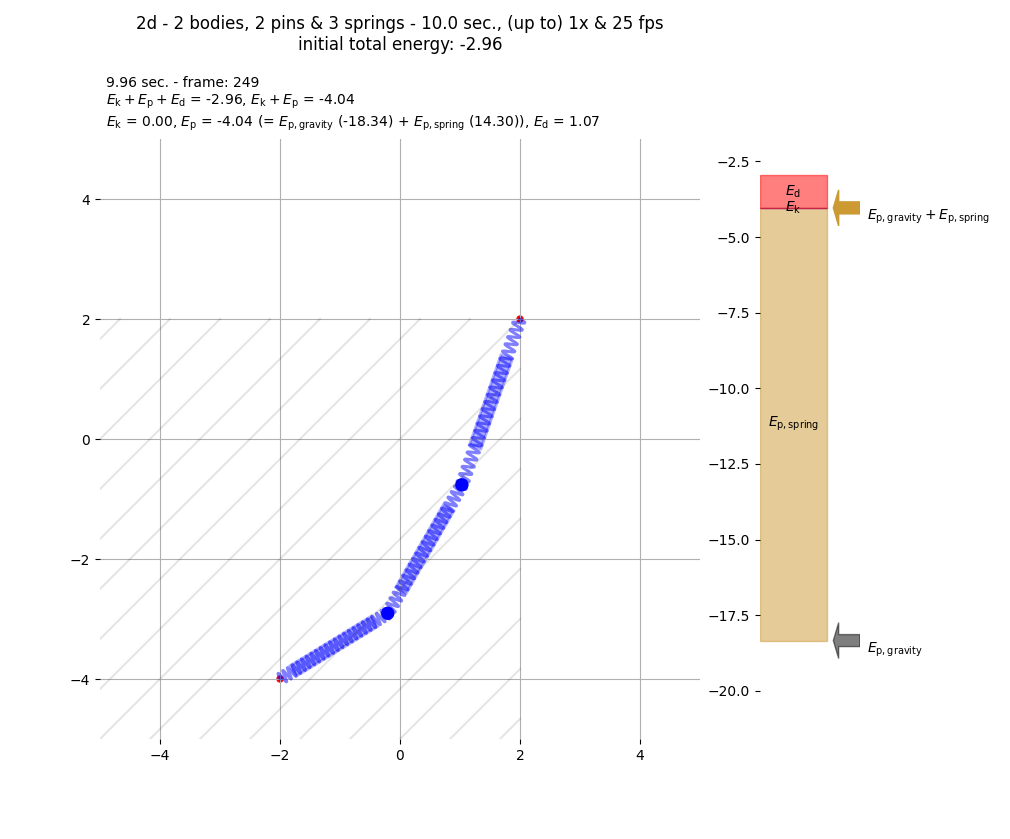
\includegraphics[trim=180 100 350 220, clip, width=.35\textwidth]{figures/2d-2-bodies-2-pins}
\end{center}
\caption{$2$ point masses and $3$ springs}
\label{fig:two-masses-and-three-springs}
\end{figure}

Note that the quantity in (\ref{eq:force:1}) equals to the sum of the forces exerted on $m_1$
and that in (\ref{eq:force:2}) equals to the sum of the forces exerted on $m_2$.
Therefore (at least for this case)
it has been shown that the configuration where the sum of all potential energies is minimized
is the same as that where the sum of the forces exerted on each mass is zero.

\subsubsection{Numerical solution}

One can solve the system of equations (\ref{eq:force:1}) and (\ref{eq:force:2})
using an iterative method such as \href{https://en.wikipedia.org/wiki/Newton%27s_method}{Netwon's method} as follows~\cite{Newton-Raphson}.
Define a function $F:\reals^6 \to \reals^6$
such that
\[
F(x) = F(x_1,x_2) = \begin{my-matrix}{c}
-\frac{\partial}{\partial x_1} f(x_1,x_2)
\\
-\frac{\partial}{\partial x_2} f(x_1,x_2)
\end{my-matrix}
\in\reals^6
\]
where $x=(x_1,x_2)\in\reals^6$
and
each term is equal to (\ref{eq:force:1}) and (\ref{eq:force:2}) respectively.
Given some initial point $x^0\in\reals^6$,
one can repeat the following procedure for $k=1,2,\ldots$
\begin{equation}
	x^{k+1} = x^k - \alpha_k DF(x^k)^{-1} F(x)
\end{equation}
where $DF:\reals^6 \to \reals^{6\times 6}$ is the Jacobian matrix of $F$
and $0<\alpha_k<1$ is step lengths for each iterate.

\subsubsection{Way easier approximate solution method}

While the function $f:\reals^6 \to\reals$ in (\ref{eq:sum-of-potential-energies}) is not a convex function,
hence it is not easy to minimize (we need some definition of \emph{easiness} here!),
we can easily, but approximately, minimize the function
by letting $l_1=l_2=l_3=0$.
If $l_1=l_2=l_3=0$,
$f$ in (\ref{eq:sum-of-potential-energies})
becomes
\begin{equation}
\label{eq:sum-of-potential-energies-convex}
\tilde{f}(x_1,x_2)
= \frac{k_1}{2} \|x_1-y_1\|^2
+\frac{k_2}{2} \|x_1-x_2\|^2
+\frac{k_3}{2} \|x_2-y_2\|^2
-a^T(m_1x_1+m_2x_2),
\end{equation}
hence a convex function~\cite{BV:04},
and the partial derivatives are
\begin{equation}
\label{eq:1}
-\frac{\partial}{\partial x_1} f(x_1,x_2) = -k_1 (x_1-y_1) -k_2(x_1-x_2) + m_1 a = 0
\in\reals^3
\end{equation}
and
\begin{equation}
\label{eq:2}
-\frac{\partial}{\partial x_2} f(x_1,x_2) = -k_2 (x_2-x_1) -k_3(x_2-y_2) + m_2 a = 0
\in\reals^3.
\end{equation}

Note that the system of equations (\ref{eq:1}) and (\ref{eq:2})
is just a linear system because they are equivalent to
\begin{equation}
\label{eq:lin-system}
\begin{my-matrix}{cc}
(k_1 + k_2)I_3 & -k_2I_3
\\
-k_2 I_3 & (k_2+k_3)I_3
\end{my-matrix}
\begin{my-matrix}{c}
x_1
\\
x_2
\end{my-matrix}
=
\begin{my-matrix}{c}
m_1a
\\
m_2a
\end{my-matrix}
\in\reals^6.
\end{equation}

Using a modern computer system and the numerical packages (that have been developed for decades by amazing experts based on amazing research results),
any linear system can be solved extremely fast, stably, and efficiently
\emph{even for hundreds of thousands of variables}.
Therefore one can obtain the solution for (\ref{eq:lin-system}) very easily.

Hence, we can use this solution for a surrogate for the equilibrium point
to find the lowest energy point fast and easily
for \emph{an arbitrarily complicated and large system}.



%\bibliographystyle{unsrt}
%\bibliographystyle{abbrv}
%\bibliographystyle{acm}
%\bibliographystyle{apalike}
%\bibliographystyle{alpha}
%\bibliographystyle{ieeetr}
\bibliographystyle{plain}
%\bibliographystyle{siam}
\bibliography{../../FrequentlyUsed/latex/mybib}

\end{document}
